\chapter{Single particle motions and radiation mechanisms}
\label{Chap:Theory:SingleParticle}

This Chapter lays the theoretical groundwork for the results presented later in this work, addressing the motion of single charged particles in electromagnetic fields, radiation mechanisms, and discussing the fundamental processes of radiation reaction and pair production.

First, equation of motions of charged single particles in electromagnetic fields are derived. This forms the basis for understanding the properties of electrons accelerated in wakefield accelerators, measuring their energy in magnetic spectrometers and calculating the radiation they emit in interaction with electromagnetic fields.

Subsequently, the production of radiation through two processes is discussed: (relativistic inverse) Compton scattering (ICS) in moderately (linear ICS) and highly intense laser fields (non-linear ICS), which is central to the work presented in Chapters \ref{Chap:linICS} and \ref{Chap:RR15}, and the radiation process of bremsstrahlung which is in particular important for the experiment outlined in Chapter \ref{Chap:BW}.

This leads over to the topic of radiation reaction, the knock-back force a charged particle experiences when emitting a photon. This can, for instance, be investigated in relativistic inverse Compton scattering. Whilst radiation reaction is a very fundamental phenomenon there is so far no universally accepted and practicable description for a wide parameter space. In this section different proposed descriptions of radiation reaction are discussed, starting with the in classical electrodynamics self-consistent Lorentz-Abraham-Dirac equation, followed by the classical Landau-Lifschitz equation and leading over to quantum corrections and their implications. 
Finally, the fundamental QED processes of pair annihilation and production through the Breit-Wheeler and Bethe-Heitler process are discussed.

\section{Single particle motion in an electromagnetic field}

The Lagrangian for a relativistic particle in an electromagnetic field with the potentials $\Phi$ and $\mathbf{A}$ is given by \cite{Jackson}
\begin{equation}
L(\mathbf{r},\mathbf{v},t) = - mc^2 \gamma^{-1}+q \mathbf{v}\cdot\mathbf{A} - q \Phi,
\end{equation}
where $m$ is the mass of the particle, $\gamma$ the relativistic Lorentz factor and $q$ the charge.
To obtain the equation of motion we use the Euler-Lagrange equation
\begin{equation}
\frac{\mathrm{d}}{\mathrm{d}t} \frac{\partial L}{\partial \mathbf{v}} - \frac{\partial L}{\partial \mathbf{r}} = 0.
\end{equation}

Using $\mathbf{A} = \mathbf{A}(\mathbf{r},t)$, $\Phi = \Phi(\mathbf{r},t)$, $\gamma^{-1} = \sqrt{1-(v/c)^2}$ and this becomes
\begin{equation}
\frac{\mathrm{d}}{\mathrm{d}t} \left[\mathbf{p}+q\mathbf{A}\right]-\left[q\nabla\left( \mathbf{A} \cdot \mathbf{v}\right) - q\nabla \Phi \right] = 0,
\label{Theory:Eqns:EoMLorentzRaw}
\end{equation}
where $\mathbf{p} = \gamma m \mathbf{v}$ is the relativistic momentum.
Now using $\frac{\mathrm{d}}{\mathrm{d}t} = \frac{\partial}{\partial t} + \mathbf{v} \cdot \nabla$ and the vector identity $\nabla \left(\mathbf{v}\cdot\mathbf{A}\right) = (\mathbf{v}\cdot\nabla)\mathbf{A} + \mathbf{v}\times(\nabla\times\mathbf{A})$ this reads:
\begin{equation}
\frac{\mathrm{d}}{\mathrm{d}t}\mathbf{p} = q\left(\mathbf{v} \times \nabla \times \mathbf{A}-\frac{\partial \mathbf{A}}{\partial t} - \nabla \Phi\right).
\label{Theory:Eqns:EoMLorentz}
\end{equation}

With the definitions of the electric field $\mathbf{E}$ and the magnetic field $\mathbf{B}$ in terms of the potentials  $\Phi$ and $\mathbf{A}$
\begin{align}
\mathbf{E} &= -\frac{\partial \mathbf{A}}{\partial t} - \nabla \Phi,\\
\mathbf{B} &= \nabla \times \mathbf{A},
\end{align}

the equation of motion takes the familiar shape of the Lorentz force:

\begin{equation}
\boxed{\frac{\mathrm{d}\mathbf{p}}{\mathrm{d}t} = q \left(\mathbf{E} + \mathbf{v} \times \mathbf{B}\right).}
\end{equation}

\subsection{Electron motion in a homogeneous electric field}

Using the previously derived equation for the Lorentz force we can now consider a first simple example. Consider the motion of a single electron in a homogeneous electric field without presence of a magnetic field, i.e. $\mathbf{B} = \mathbf{0}$. The Lorentz equation simplifies to:

\begin{equation}
\frac{\mathrm{d}\mathbf{p}}{\mathrm{d}t} = q \mathbf{E}.
\end{equation}

If we choose the coordinate system such that  $\mathbf{E} =  (E,0,0)^t = E \mathbf{e}_x$, the electron feels a constant force $qE$ accelerating it in $x$ at a linear energy gain. Its momentum, however, is unchanged in the other two directions, $\mathrm{d}p_x/\mathrm{d}t = \mathrm{d}p_y/\mathrm{d}t = 0$. 

\subsection{Electron motion in a homogeneous magnetic field}

Consider the motion of a single electron in a homogeneous magnetic field extending over the entire region of interest. The equation for the Lorentz force simplifies with $\mathbf{E} = \mathbf{0}$ to:
\begin{subequations}
\begin{align}
\frac{\mathrm{d}\mathbf{p}}{\mathrm{d}t} &= q \mathbf{v} \times \mathbf{B},\\
\frac{\mathrm{d}\mathbf{p}}{\mathrm{d}t} &= \frac{q}{\gamma m} \mathbf{p} \times \mathbf{B},
\end{align}
\end{subequations}
in terms of the relativistic momentum $\mathbf{p} = \gamma m \mathbf{v}$.
Note that in this case the purely magnetic Lorentz force does not do any work. The instantaneous rate of work (power) is $P = \mathbf{F} \cdot \mathbf{v}$, where the force $\mathbf{F}$ is by virtue of the cross product always orthogonal to $\mathbf{v}$ and the dot product vanishes.
We choose the coordinate system such that $\mathbf{B} = (0,0,B)^t = B e_z$. The momentum vector is simply $\mathbf{p} = (p_x,p_y,p_z)^t$.
The differential equations are then given by:
\begin{subequations}
\begin{align}
\dot{p_x} &= \frac{qB}{\gamma m} p_y,\\
\dot{p_y} &= - \frac{qB}{\gamma m} p_x,\\
\dot{p_z} &= 0,
\end{align}
\end{subequations}
which combines to
\begin{subequations}
\begin{align}
\ddot{p_x}  &= - \left(\frac{qB}{\gamma m}\right)^2 p_x,\\
\ddot{p_y}  &= - \left(\frac{qB}{\gamma m}\right)^2 p_y.
\end{align}
\end{subequations}
This second order, linear differential equation can be solved by a periodic motion of type $p_x(t) = C \sin(\omega t) + D \cos(\omega t)$ with $\omega = qB/\gamma m$. The dotted variables indicate the time derivatives with $\dot{p} = \mathrm{d}p/\mathrm{d}t$ and $\ddot{p}=\mathrm{d}^2p/\mathrm{d}^2t$.

$\mathbf{p_\perp}$ be the momentum vector of the particle perpendicular to the magnetic field lines and $\mathbf{p_\parallel}$ the component parallel to the magnetic field (z). For the initial conditions $p_x(t=0) = |\mathbf{p_\perp}| = p_\perp$ and $p_y(t=0)=0$, we obtain for the momenta:
\begin{subequations}
\begin{align}
p_x(t) &= p_\perp \cos(\omega t)\\
p_y(t) &= - p_\perp \sin(\omega t) 
\end{align}
\end{subequations}
The solution for the $z$-motion is trivial with $p_z = p_{z,0}$.
Expressed in terms of the trajectories with initial conditions $x(0) = 0, z(0) = 0, y(0) = p_\perp/qB = r_{L}$, this reads
\begin{subequations}
\begin{empheq}[box=\widefbox]{align}
x(t) &= r_{L} \sin(\omega t)\\
y(t) &= r_{L} \cos(\omega t)\\
z(t) &= \frac{p_{z,0}}{\gamma m} t
\end{empheq}
\end{subequations}

The radius of the circular motion of the electron is called the Larmor radius $r_L$. It depends on the total momentum in the $x$-$y$ plane and the magnetic field strength $B$: 
\begin{equation}
\boxed{r_{L} = |\mathbf{p}_\perp|/eB,}
\end{equation}
where $e$ is the charge of the electron and $\mathbf{p}_\perp$ is the component of the momentum vector $\mathbf{p}$ that is perpendicular to the field component of the magnetic field.
\vspace{\baselineskip}

The motion of the electron consists of two decoupled motions: one at the constant, initial velocity parallel to the magnetic field vector in $z$, the second motion is a circular motion in the $x$-$y$ plane. This is called a cyclotron motion. For now we will ignore the dissipation of energy in form of radiation due to the acceleration of the electron and accept the result that the Lorentz force conserves the total momentum and energy of the particle in this case.

\subsection{Electron motion in a monochromatic plane EM wave}
\label{Theory:Sec:SingleParticle:FigOfEight}

We will now consider the case of an electron in a monochromatic plane wave.
Writing the equation of motion in terms of the potentials $\mathbf{A}$ and $\Phi$ as in Equation \eqref{Theory:Eqns:EoMLorentz} on page \pageref{Theory:Eqns:EoMLorentz} gives \cite{ThomasThesis}:

\begin{equation}
\frac{\mathrm{d}}{\mathrm{d}t}\mathbf{p} = q\left(\mathbf{v} \times \nabla \times \mathbf{A}-\frac{\partial \mathbf{A}}{\partial t} - \nabla \Phi\right).
\end{equation}

Now using the convective derivative, $\mathrm{d}\mathbf{p}/\mathrm{d}t = \partial \mathbf{p}/\partial t + \mathbf{v} \cdot \nabla \mathbf{p}$ and the vector identity $\mathbf{v} \cdot \nabla \mathbf{p} = (\nabla \mathbf{p})\cdot\mathbf{v} - \mathbf{v} \times (\nabla\times\mathbf{p})$ again, the total time derivative of the momentum expands to
\begin{equation}
\frac{\mathrm{d}}{\mathrm{d}t}\mathbf{p} = \frac{\partial\mathbf{p}}{\partial t} +(\nabla\mathbf{p})\cdot\mathbf{v} - \mathbf{v}\times(\nabla\times\mathbf{p}).
\end{equation}
With this result the equation of motion becomes
\begin{align}
\frac{\partial\mathbf{p}}{\partial t} +(\nabla\mathbf{p})\cdot\mathbf{v} - \mathbf{v}\times(\nabla\times\mathbf{p}) &= q\left(\mathbf{v} \times \nabla \times \mathbf{A}-\frac{\partial \mathbf{A}}{\partial t} - \nabla \Phi\right),\nonumber\\
\frac{\partial}{\partial t}\left(\mathbf{p}+q\mathbf{A}\right) +(\nabla\mathbf{p})\cdot\mathbf{v} - \mathbf{v}\times\left(\nabla\times\left(\mathbf{p}+q\mathbf{A}\right)\right) &= - q\nabla \Phi,\nonumber\\
\frac{\partial}{\partial t}\mathbf{u} +(\nabla\mathbf{p})\cdot\mathbf{v} - \mathbf{v}\times\left(\nabla\times\mathbf{u}\right) &= - q\nabla \Phi,
\label{Theory:Eqns:EoMLaserAT}
\end{align}
where we introduced in the last step the canonical momentum $\mathbf{u} = \mathbf{p} + q\mathbf{A}$.
We can express $(\nabla\mathbf{p})\cdot \mathbf{v}$ as follows
\begin{equation}
(\nabla\mathbf{p})\cdot \mathbf{v} = \frac{1}{m\gamma} \nabla (p^2/2) = \frac{1}{m\gamma}\nabla(\gamma^2/2) = m c^2 \nabla \gamma.
\label{Theory:Eqns:nablaDotV}
\end{equation}

Substituting $(\nabla\mathbf{p})\cdot \mathbf{v}$ in Equation \eqref{Theory:Eqns:EoMLaserAT} by the expression in Equation \eqref{Theory:Eqns:nablaDotV}:
\begin{equation}
\frac{\partial}{\partial t}\mathbf{u} = \mathbf{v}\times\left(\nabla\times\mathbf{u}\right) - \nabla \left(q\Phi + \gamma mc^2\right).
\label{Theory:Eqns:partialtU}
\end{equation}

Taking the curl of this equation results in:
\begin{equation}
\frac{\partial}{\partial t}\nabla\times\mathbf{u} = \nabla\times\left[\mathbf{v}\times\left(\nabla\times\mathbf{u}\right)\right],
\end{equation}
where the second term disappeared as the curl of a gradient is always zero,
so that if $\nabla \times \mathbf{u}$ is zero initially, it will remain so always. The condition is satisfied, for instance, for a plasma at rest before the laser pulse arrives.
Assuming this condition Equation \eqref{Theory:Eqns:partialtU} simplifies to
\begin{equation}
\frac{\partial}{\partial t}\mathbf{u} = - \nabla \left(q\Phi + \gamma mc^2\right).
\end{equation}

For a medium close to vacuum or an unperturbed plasma one can assume $\Phi = 0$, resulting in:
\begin{equation}
\frac{\partial}{\partial t}\mathbf{u} =  -\nabla\gamma mc^2.
\end{equation}
In the case of an infinite plane wave the transverse gradient $\nabla_\perp$ is zero.
This means we obtain two separate components:
\begin{subequations}
\begin{align}
\frac{\partial}{\partial t}\mathbf{u}_\perp &= 0,\\
\frac{\partial}{\partial t}\mathbf{u}_\parallel &= \nabla_\parallel \gamma mc^2.
\end{align}
\end{subequations}

From the perpendicular component we see that the transverse canonical momentum is conserved: $\mathbf{p}_\perp + q\mathbf{A} = 0$. If $q = -e$ and $e\mathbf{A}_\perp = \mathbf{a}_\perp$, then $\mathbf{p}_\perp = \mathbf{a}_\perp$. In Cartesian coordinates, this means $p_x = a_x, p_y = a_y$.

For the parallel spatial component $z$ consider the substitution $z = ct$ for light. Thus, $\partial z = c \partial t$. The parallel-component of the vector potential $\mathbf{A}$ is zero, so $u_\parallel = p_\parallel = p_z$:
\begin{equation}
\frac{\partial}{\partial t}(cp_z - \gamma mc^2) = 0.
\end{equation}

Assuming an unperturbed stationary plasma, the initial conditions are $\gamma(t=0) = 1$ and $p_z(t=0) = 0$. Integrating the previous equation gives:
\begin{equation}
c p_z+ mc^2 = \gamma mc^2.
\end{equation}

Using $E = \gamma m c^2 = \sqrt{mc^2 + (cp_\parallel)^2 + (cp_\perp)^2}$ and substituting, one obtains an expression for $p_\parallel = p_z$:

\begin{equation}
p_z = \frac{1}{2} mc a^2,
\end{equation}
where $a^2 = p^2_\perp$.
We now have
\begin{subequations}
\begin{align}
p_x &= mc a_x,\\
p_y &= mc a_y,\\
p_z &= \frac{1}{2} mc a^2.
\end{align}
\end{subequations}

Using $\mathbf{p} = \gamma m \mathbf{v}$ this can be written as:
\begin{subequations}
\begin{align}
\frac{\gamma}{c} \frac{\mathrm{d}x}{\mathrm{d}t} &= a_x,\\
\frac{\gamma}{c} \frac{\mathrm{d}y}{\mathrm{d}t} &= a_y,\\
\frac{\gamma}{c} \frac{\mathrm{d}z}{\mathrm{d}t} &= \frac{a^2}{2}.
\end{align}
\end{subequations}

Changing from $t$ to proper time $\tau$, we transform via $\mathrm{d}\tau = \gamma^{-1}\mathrm{d}t$, simply giving the equation of motions in term of $\tau$:
\begin{subequations}
\begin{align}
\frac{1}{c}\frac{\mathrm{d}x}{\mathrm{d}\tau} &= a_x,\\
\frac{1}{c}\frac{\mathrm{d}y}{\mathrm{d}\tau} &= a_y,\\
\frac{1}{c}\frac{\mathrm{d}z}{\mathrm{d}\tau} &= \frac{a^2}{2}.
\end{align}
\end{subequations}

Let us assume a laser field with linear polarisation in $x$, described by the vector potential
\begin{equation}
\mathbf{a} = a_0 \cos(kz - \omega t)\mathbf{e}_x = a_0 \cos(\xi)\mathbf{e}_x,
\end{equation}
where $\mathbf{e}_x$ is the unit vector in the $x$-coordinate, $\xi = kz - \omega t$ the waveframe coordinate and $k = \omega/c$ the wave number. 

\begin{figure}[h]
\centering
	\includegraphics[width=0.49\columnwidth]{figeight_lab.pdf}
	\includegraphics[width=0.49\columnwidth]{figeight_drift.pdf}
\caption[Electron motion in an infinite, linearly polarised, plane EM wave.]{Electron motion in an infinite, linearly polarised, plane EM wave in the lab frame (left), with the wavenumber $k = \omega/c$. On the right the figure-of-eight motion in the drift frame.}
\label{Theory:Figs:FigureOfEight}
\end{figure}

Using this explicit vector potential:
\begin{subequations}
\begin{align}
\frac{\gamma}{c}\frac{\mathrm{d}x}{\mathrm{d}t} &= a_0 \cos \xi,\\
\frac{\gamma}{c}\frac{\mathrm{d}y}{\mathrm{d}t} &= 0,\\
\frac{\gamma}{c}\frac{\mathrm{d}z}{\mathrm{d}t} &= \frac{1}{2} a^2_0 \cos^2 \xi.
\end{align}
\end{subequations}

and integrating the equation of motions, results in:
\begin{subequations}
\begin{align}
x(\xi) &= \frac{a_0}{k}\sin(\xi),\\
y(\xi) &= 0,\\
z(\xi) &= \frac{a^2_0}{4k}\left(\xi + \frac{1}{2}\sin(2\xi)\right),
\end{align}
\end{subequations}
where we chose the initial conditions $x(0)=y(0)=z(0)=0$  and used $\mathrm{d}\xi/\mathrm{d}t = \omega/\gamma$.
The electron performs a periodic oscillation in the $x$-axis, whilst the motion in the $z$-axis is composed of a constant drift and another oscillation (see Figure \ref{Theory:Figs:FigureOfEight} (left)). This is commonly referred to as the `figure-of-eight' motion, which becomes more evident in the drift frame (see Figure \ref{Theory:Figs:FigureOfEight} (right)). For $a_0 \leq 1$ the motion in $z$ is suppressed and the motion of the electron is dominated by the transverse oscillation. For $a_0 \gg 1$, the motion is predominantly longitudinal.





\subsection{Ponderomotive Force}
\label{Theory:Sec:PonderomotiveForce}

In laser wakefield acceleration (LWFA) a high intensity laser pulse propagates through an underdense plasma, expels electrons in its way and drives a wave. The driving force is the so-called ponderomotive force which is proportional to the gradient of the laser intensity. 

The following relativistic derivation of the ponderomotive force is based on \cite{ThomasThesis}.
We start with the Euler-Lagrange equations after inserting the Lagrangian in terms of the potentials $\mathbf{A}$ and $\Phi$ as given as intermediate step in Equation \eqref{Theory:Eqns:EoMLorentzRaw} on page \pageref{Theory:Eqns:EoMLorentzRaw}:
\begin{equation}
\frac{\mathrm{d}}{\mathrm{d}t} \left[\mathbf{p}+q\mathbf{A}\right]-\left[q\nabla\left( \mathbf{A} \cdot \mathbf{v}\right) - q\nabla \Phi \right] = 0.
\end{equation}

This can be written in terms of the normalised quantities
\begin{align}
\mathbf{a} &= -q \mathbf{A}/m_e c, & \phi &= -q\phi/mc^2,\nonumber\\
\mathbf{v} &\rightarrow \beta = \mathbf{v}/c, & \mathbf{p} &\rightarrow \mathbf{p}/m c,
\end{align}

resulting in
\begin{equation}
\frac{\mathrm{d}}{\mathrm{d}t} \left[\mathbf{p}-\mathbf{a}\right] - \left(c\nabla \mathbf{a}\right) - c \nabla \phi = 0.
\end{equation}

Using the canonical momentum $\mathbf{u} = \mathbf{p} - \mathbf{a}$ the time derivative can now be re-written and we can also substitute $\mathbf{v} = \mathbf{p}/\gamma = (\mathbf{u}+\mathbf{a})/\gamma$:
\begin{align}
\frac{\mathrm{d}}{\mathrm{d}t}\mathbf{u} &= c\nabla\phi - (c\nabla\mathbf{a})\cdot\frac{(\mathbf{u}+\mathbf{a})}{\gamma},\nonumber\\
\frac{\mathrm{d}}{\mathrm{d}t}\mathbf{u} &= c\nabla\phi - \frac{1}{\gamma} c \nabla \frac{\mathbf{a}^2}{2}-c\nabla\mathbf{a}\cdot\frac{\mathbf{u}}{\gamma}.
\end{align}

In the scenario of an electromagnetic pulse at high frequency $\omega$ of long pulse duration $\tau \gg 1/\omega$ and sufficiently large spot size $w \gg 1/|k|$ in terms of the fast oscillations, fast and slow dynamics can be treated separately.
When averaging over the time of a period $T = 2\pi/\omega$, the terms of linear order $\mathbf{a}$ and the potential $\phi$ amount to zero:
\begin{equation}
\boxed{\left\langle\frac{\mathrm{d}}{\mathrm{d}t}\mathbf{u}\right\rangle \sim -\left\langle\frac{1}{\gamma}c\nabla\frac{\mathbf{a}^2}{2}\right\rangle,}
\end{equation}

which is the ponderomotive force $\mathbf{F}_p$ acting on a single electron. Since $\mathbf{F}_p \sim \nabla \left\langle\mathbf{a}^2\right\rangle$, this implies $\mathbf{F}_p \sim \nabla \left\langle I\right\rangle$, i.e. the ponderomotive force pushes electrons away from regions of high intensity and is hence a suitable force to drive LWFA.

On the other hand, the ponderomotive force is suppressed for ultrarelativistic particles as $1/\gamma \ll 1$ as considered in relativistic inverse Compton scattering geometries as used in studies of radiation reaction (see Chapters \ref{Chap:linICS}, \ref{Chap:RR15} and \cite{Cole2018_RR,Poder2018_RR,Burke1997_RR,Bula1996_RR}).


\section{Radiation Production}


In the previous sections we discussed the motion of single particles in electromagnetic fields, followed by an introduction in the dynamics of lasers, plasmas and their interplay to produce relativistic electron beams. In the following we will consider the production of radiation through different mechanisms.

\begin{itemize}
\item two methods to calculate the radiation spectra, cross sections and so on:
\item classical method is deriving the equation of motion, analyse in terms of Lienard-Wiechert potentials and solve the radiation integrals.
\item Fourier analysis tells us the spectrum and the cross sections.
\item in the quantum picture the cross sections and spectra are obtained by solving the Feynman diagrams related to the process
\item however, at higher intensities the number of contributing diagrams increases significantly, so that the standard Feynman diagrams are replaced by `dressed states' which replace electrons interacting with photons by electrons in background fields.
\item this is referred to as the Furry picture. Here the dressed states use an exact description (classical) of the background fields.
\item This is in particular important in the high-field regimes as the sum of infinite Feynman diagrams is equivalent to the Volkov states.
\end{itemize}


\begin{figure}
\centering
\includegraphics[height=.3\columnwidth]{Aivazis_ComptonScattering_FULL.pdf}

\includegraphics[height=.3\columnwidth]{Aivazis_ComptonScattering2_FULL.pdf}

\includegraphics[height=.3\columnwidth]{feyn_nICS.pdf}
\caption{Feynman diagram for Volkov state equivalent to infinite series of diagrams}
\label{Theory:Figs:HighFieldProcess}
\end{figure}


The first radiation sources considered are synchrotron radiation with the special case of undulator and wiggler radiation, where a magnetic field or a series of alternating magnetic fields oscillates the particles to produce radiation. This section is followed by betatron radiation where the magnetic field is replaced by an electric field in the cavity of the wakefield accelerator, sometimes referred to as a plasma wiggler. In both scenarios the electrons perform figure-of-eight motions as outlined in Section XX\addnum{}, and the the emission spectra follow accordingly similar equations where the wiggler parameter, $K$ and $K_\beta$, indicate the properties.

We then investigate Compton scattering and its classical low-limit Thomson scattering, where a photon scatters off an electron at rest. After deriving the cross section and energy spectra we consider the special case of inverse Compton scattering, where the photon scatters from a relativistic electron and the radiation gains a significant amount of energy proportional to the electron energy due to the relativistic Doppler effect. At high field strengths multiple photons can interact in a nonlinear interaction to produce higher harmonic radiation, called nonlinear inverse Compton scattering or relativistic nonlinear Thomson scattering. The trajectories of the electrons in these processes are also described by a figure-of-eight motion as the electrons are now in a laser wiggler, where the wiggler parameter, $K$, is replaced by the normalised vector potential, $a_0$.

Finally, we will introduce the process of bremsstrahlung where electrons interact with the nuclear Coulomb field to produce X-ray and gamma radiation.

A review of radiation mechanisms and sources in the context of wakefield accelerators can be found in \cite{Corde2013_Rad} and \cite{Albert2016_APP}.
A review particularly aimed at high-field interactions \cite{DiPiazza2012_ICS}

\subsection{Compton Scattering}

\textit{Compton scattering} describes the inelastic scattering of a photon off a charged free or quasi-free particle, typically an electron \cite{Compton1923_Compton,Klein1929_KNEq}. The photon transfers energy to the electron and as a result loses energy. In the low energy limit of the photon energy $\omega \rightarrow 0$ the interaction becomes fully elastic and is called \textit{Thomson scattering} \cite{Thomson2005_ThomsonScatter}, i.e. Thomson scattering is the low-energy classical limit of Compton scattering.
The interaction can be written as follows:
\begin{equation}
\gamma + e^- \longrightarrow \gamma + e^-,
\end{equation}
with the corresponding Feynman diagram shown in Figure \ref{Theory:Fig:ComptonScattering:Feynman}.
\begin{figure}[h]
\centering
\includegraphics[width=0.5\columnwidth]{Aivazis_ComptonScattering.pdf}
\caption[Feynman diagram for Compton scattering.]{Feynman diagram for Compton scattering. The time axis is oriented from left to right. Wiggly lines indicate photons, the arrowed lines represent fermions (arrow towards positive time), here electrons.}
\label{Theory:Fig:ComptonScattering:Feynman}
\end{figure}


\subsubsection{Kinematics}

\begin{figure}
\centering
\includegraphics[width=0.8\columnwidth]{Compton_kinematics_sketch.pdf}
\caption[Kinematics diagram for Compton scattering.]{Sketch of the kinematics for Compton scattering. A photon of energy $E_{\gamma,i}$ (green) is incident onto an electron at rest (blue), i.e. $E_{e,i} = m_e c^2$, and scatters off it at an angle $\theta$. The electron is scattered at an angle $\phi$. The photon and the electron exchange momentum.}
\label{Theory:Fig:ComptonScattering:Kinematics}
\end{figure}

In the following, we will treat the electron and the incoming photon both as particles and calculate their final momenta based on energy and momentum conservation in a relativistic framework.
\vspace{\baselineskip}

Assuming the electron has a negligible initial momentum $\mathbf{p}_{e,i} = \mathbf{0}$ as in Compton's original experiment \cite{Compton1923_Compton}, the total energy hence reduces to the rest energy of the electron $E_{e,i} = m_e c^2$. The subscript $e$ stands for `electron' and $i$ for `initial'.
The photon on the other hand has an initial momentum $\mathbf{p}_{\gamma, i}$ and an energy $E_{\gamma, i} = p_{\gamma, i} c = hf$, where $h$ is Planck's constant and $f$ the frequency of the photon. The subscript $\gamma$ represents the photon in this interaction.
Relying on the conservation of energy we can postulate that the sum of energies before and after the interaction have to be equal:
\begin{align}
E_{e, i} + E_{\gamma,i} &= E_{e,f} + E_{\gamma,f},\nonumber\\ 
m_e c^2 + h f &= \sqrt{(p_{e,f} c)^2 + (m_e c^2)^2} + h f',\nonumber\\
hf - hf' +m_e c^2 &= \sqrt{(p_{e,f} c)^2 + (m_e c^2)^2},\nonumber\\
\left( hf - hf' +m_e c^2\right)^2 -(m_e c^2)^2 &= (p_{e,f} c)^2, \nonumber\\
(E_{\gamma, i} - E_{\gamma, f} + m_e c^2)^2 - (m_e c^2)^2 &= (p_{e, f} c)^2,
\label{Theory:Eqns:Compton_EnergyConserve}
\end{align}
where $f'$ is the frequency of the photon after the interaction.
Similarly, we can use momentum conservation to find an expression for the momentum of the electron after the scattering:
\begin{align}
\mathbf{p}_{\gamma, i} &= \mathbf{p}_{e, f} + \mathbf{p}_{\gamma, f}\nonumber\\
\mathbf{p}_{\gamma, i} - \mathbf{p}_{\gamma, f} &= \mathbf{p}_{e, f}\nonumber\\
(\mathbf{p}_{\gamma, i} - \mathbf{p}_{\gamma, f})^2 &= (\mathbf{p}_{e, f} )^2\nonumber\\
(p_{\gamma, i}c)^2 + (p_{\gamma, f}c)^2 - 2 p_{\gamma, i}p_{\gamma, f}c^2\cos\theta &= (p_{e, f} c )^2,\nonumber\\
E_{\gamma, i}^2 + E_{\gamma, f}^2 - 2 E_{\gamma, i} E_{\gamma, f} \cos\theta &= (p_{e, f} c)^2,
\label{Theory:Eqns:Compton_MomConserve}
\end{align}
where $\mathbf{p}$ is a momentum vector and $|\mathbf{p}| = p$ its corresponding length. $\theta$ is the angle between incoming and outgoing momentum vector of the photon (see Figure \ref{Theory:Fig:ComptonScattering:Kinematics}).
Setting Equations \eqref{Theory:Eqns:Compton_EnergyConserve} and \eqref{Theory:Eqns:Compton_MomConserve} equal we find the familiar equation for the angular dependent change in wavelength of a photon performing Compton scattering with an electron:
\begin{equation}
\lambda_{final} - \lambda_{initial} = \frac{h}{m_e c} \left(1 - \cos\theta\right) = \lambda_C \left(1-\cos\theta\right),
\end{equation}
where $\lambda_C = hm_e c$ is the Compton wavelength.
Similarly there is an equation for the emission angle of the electron:
\begin{equation}
\cot(\phi) = \left(1+\frac{hf}{m_e c^2}\right) \tan(\theta/2).
\end{equation}

In terms of photon energy we can write
\begin{equation}
\boxed{E_{\gamma,f} = \frac{E_{\gamma,i}}{1+\frac{E_{\gamma,i}}{m_e c^2}(1-\cos\theta)},}
\label{Theory:Eqs:Compton_Egammaf}
\end{equation}
where the final energy, $E_{\gamma,f}$, only depends on the energy of the incoming photon, $E_{\gamma,i}$, and the scattering angle $\theta$. 
Polar plots of the final photon energies for different initial photon energies are shown in Figure \ref{Theory:Figs:Compton_E_XSEC} (left). At low energies $E_{\gamma,i} \rightarrow 0$ and $E_{\gamma,f} \rightarrow E_{\gamma,i}$, and the emitted energy becomes approximately independent of the scattering angle $\theta$ (see Figure \ref{Theory:Figs:Compton_E_XSEC} (left, inset)). At higher energies $E_{\gamma,i} > m_e ^2c$, the energy distribution is being skewed towards the forwards direction of the incoming photon and the energy of the photon after the interaction is maximised at zero degrees with $E_{\gamma,f} = E_{\gamma,i}$, i.e. no significant amount of energy is transferred to the electron (see Figure \ref{Theory:Figs:Compton_E_XSEC} (left)).


\subsubsection{Cross-Section}


\begin{figure}
\centering
\includegraphics[width=.5\columnwidth]{Compton_kinematic.pdf}\includegraphics[width=.5\columnwidth]{Compton_KN_cross.pdf}
\caption[Polar plot of photon energies and related differential cross section for Compton scattering.]{Left: Polar plot of photon energies after Compton scattering from an electron at rest for different incoming photon energies (legend) for up to 100 keV (left, inset) and up to 10 MeV (left). The incoming photon travels on the zero degree axis. The energy axis is linear and the numbers show the energy in MeV. Right: Polar plot of the differential cross section in arbitrary units for photon scattering angles calculated using Equation \eqref{Theory:Eqs:ComptonXsec} for different initial photon energies (legend).}
\label{Theory:Figs:Compton_E_XSEC}
\end{figure}

The cross section for Compton scattering, again assuming the electron is initially at rest, is given by the spin-averaged Klein-Nishina formula \cite{Klein1929_KNEq} (see Section \ref{Appendix:QEDDeriv_KleinNishina} for an explicit derivation and the spin-dependent equation):
\begin{subequations}
\begin{empheq}[box=\widefbox]{align}
\frac{\mathrm{d}\sigma_{\gamma e}}{\mathrm{d}\cos{\theta}} &= \pi r^2_e \left(\frac{\omega'}{\omega}\right)^2 \left(\frac{\omega'}{\omega} + \frac{\omega}{\omega'}-\sin^2{\theta}\right),\\
\frac{\mathrm{d}\sigma_{\gamma e}}{\mathrm{d}\cos{\theta}} &= \pi r^2_e  \left(\frac{E_f}{E_i}\right)^2 \left(\frac{E_f}{E_i} + \frac{E_i}{E_f}-\sin^2{\theta}\right),
\end{empheq}
\label{Theory:Eqs:ComptonXsec}
\end{subequations}
in terms of the initial and final frequency and energy, respectively.
For very low energetic photons in the limit $\omega \rightarrow 0$ and $\omega'/\omega \rightarrow 1$ the cross section simplifies to 
\begin{equation}
\boxed{\frac{\mathrm{d}\sigma_{\gamma e}}{\mathrm{d}\cos{\theta}} = \pi r^2_e (1 + \cos^2\theta),}
\label{Theory:Eqs:ThomsonXsec}
\end{equation}
which is independent of photon energy and has a total cross section of $\sigma_{\gamma e} = \sigma_T = 8\pi r^2_e/3 $, with $r_e = e^2/4\pi \epsilon_0 m_e c^2 = 6.65 \times 10^{-29}\,\mathrm{m}^2$ \cite{Jackson}. This is the classical Thomson scattering cross section, $\sigma_T$.
The total cross section using the Klein-Nishina equation amounts to:
\begin{equation}
\boxed{\sigma_{\gamma e} = 2\pi r^2_e \left[\frac{1 + x}{x^3}\left( \frac{2x(1+x)}{1+2x} - \ln(1+2x)\right) + \frac{1}{2x} \ln(1+2x) - \frac{1+3x}{(1+2x)^2}\right],}
\end{equation}
with $x = E_\gamma /m_e c^2$, so that in the two limits this becomes
\begin{equation}
\sigma_{\gamma e} = \sigma_T \times  
\begin{cases}
(1-2x+\frac{26 x^2}{5}) & \mathrm{for }~x\ll1,\\
\frac{3}{8}\frac{1}{x} \left( \ln 2x + \frac{1}{2}\right) & \mathrm{for }~x\gg 1,
\end{cases}
\end{equation}
so that $\sigma_{\gamma e} \rightarrow \sigma_T$ for $x \rightarrow 0$, which is the limit of Thomson scattering, and $\sigma_{\gamma e} \rightarrow 0$ for $x\rightarrow \infty$, which indicates that ultra-relativistic photons are less likely to scatter.

The differential cross section is shown in a polar plot in Figure \ref{Theory:Figs:Compton_E_XSEC} (right) for different incoming photon energies. At low photon energies the cross section and the photon spectrum are symmetric in forwards and backwards direction following Thomson scattering (see Equation \eqref{Theory:Eqs:ThomsonXsec}). At increasing photon energies reaching the X-ray and gamma regime the photon is preferentially scattered in the forwards direction at lower momentum transfers and falling to $0$ at $\theta = 0$.

\subsection{Linear Inverse Compton Scattering}
\label{Theory:Sec:LinearICS}

In the previous section Compton scattering and its classical low-energy limit Thomson scattering were discussed for a single photon interacting with an electron that is initially at rest. Here we will consider the special case of a relativistic electron of energy $\epsilon \gg m_e c^2$ interacting with a single photon. Whilst in `standard' Compton scattering momentum is transferred from the photon to the electron, resulting in a longer wavelength of the scattered photon, we will see that in this scenario the photon gains considerable amount of energy from the electron. Due to this inversion of the energy balance relative to standard Compton scattering, this special case is referred to as \textit{inverse} Compton scattering (ICS). In the limit discussed here it is also referred to as relativistic Thomson scattering or Compton backscattering. In this section we will neglect nonlinear effects such as the emission of higher harmonics or the relativistic mass gain of electrons in an intense laser field. These phenomena will be discussed in the following section related to nonlinear inverse Compton scattering.

\subsubsection{Kinematics}

To treat this scattering process similarly to the standard Compton scattering discussed in the previous section, we will shift to the rest frame of the electron, where the initial condition, that the electron is at rest, is again satisfied. In the following, quantities in the lab frame, $S$, will be denoted as before, for instance $E, \theta$. In the rest frame of the electron, $S'$, quantities will be denoted as dashed quantities, i.e. $E', \theta'$ and so on.

Assume a single relativistic electron with a relativistic Lorentz factor, $\gamma$, moving in $x$ and a photon of energy $E_{i}$ with an incident angle $\theta_i$ relative to this axis.
In the rest frame of the electron the photon experiences a relativistic Doppler-shift so that its energy in this frame, $E'_{i}$, is
\begin{equation}
E'_i = \gamma E_i (1-\mathbf{\beta} \cdot \mathbf{e_k}) = \gamma E_i (1 - \beta \cos\theta) \approx \gamma E_i (1- \cos\theta),
\end{equation}
where we assumed that the electron is highly relativistic and $\beta \approx 1$.
In a head-on collision ($\theta = \pi$) the photon energy in the electron rest frame is maximised by a factor of $2\gamma$. The angles transform via
\begin{equation}
\sin\theta' = \frac{\sin \theta}{\gamma (1 + \beta \cos \theta)},~\cos \theta' = \frac{\cos \theta + \beta}{1 + \beta \cos \theta}.
\label{Theory:Eqs:ICS:BoostAngles}
\end{equation}

In this frame the scattered photon energies follow the same relation as for standard Compton scattering (see Equation \eqref{Theory:Eqs:Compton_Egammaf}), but in terms of dashed quantities:
\begin{equation}
E'_f = \frac{E'_i}{1+\frac{E'_i}{m_e c^2}(1-\cos\alpha')},
\end{equation}
where $\alpha'$ is the difference between the incident and outgoing angle and determined by
\begin{equation}
\cos \alpha' = \mathbf{n'_f} \cdot \mathbf{n'_i} = \cos \theta'_i \cos \theta'_f + \sin \theta'_i \sin \theta'_f \cos(\phi'_i - \phi'_f),
\end{equation}
with the angles $\phi'$ denoting the azimuthal angles of the photon. 
In this frame the photon is losing energy as it transfers momentum to the electron, as expected for Compton scattering. In a head-on collision in the lab frame for $\gamma \sim 1000$ and $E_i = 1\eV$, the energy in the electron rest frame becomes $E'_i = 2\keV$, with $E'_i \ll m_e c^2$ or in terms of lab-frame quantities $E_i \ll m_e c^2/\gamma$. This means that under these conditions this interaction corresponds to Thomson scattering. 

In order to calculate the final photon energy in the laboratory frame, $S$, we have to boost back from the rest frame of the electron, $S'$, which results in another amplifying factor of $\sim\gamma$:
\begin{equation}
E_f = E'_f \gamma (1+\beta \cos \theta'_f) \approx E'_f \gamma (1+ \cos \theta'_f) \propto \gamma^2 E_i,
\end{equation}
where the angles have to be transformed back into the lab frame as well. We now see that in the lab frame $E_f > E_i$, so that the photon gains energy in the interaction and the name \textit{inverse} Compton scattering is justified.
The emitted energy is maximised in a head-on collision and when radiated in the propagation direction of the relativistic electron.
The photon energy is then boosted by $(2\gamma)^2$ to $E_{f,max} = 2 \gamma E'_f = 2 \gamma E'_i = 4 \gamma^2 E_i$. In the rest frame of the electron this corresponds to $E'_i = E'_f$, which again indicates Thomson scattering and motivates another common name for this process, \textit{relativistic Thomson scattering}.

\subsubsection{Cross-Section}

$E_i = m_e c^2/\gamma$ would for $E_i = 1\eV$ require $\gamma \sim 5\times 10^5$ or $\epsilon \sim 250\GeV$.  As a result, $E_i \ll m_e c^2/\gamma$ holds for all relevant scenarios and the interaction is in the rest frame accurately described by the Thomson cross section as given in Equation \eqref{Theory:Eqs:ThomsonXsec}, but in quantities of the rest frame $S'$:
\begin{equation}
\frac{\mathrm{d} \sigma'}{\mathrm{d}\cos \theta'} =\pi r^2_e \left(1+\cos^2 {\theta'}\right).
\end{equation}

For $\gamma \gg 1$ the transformation of the angles results in the so-called `headlight' or `searchlight effect' since $\cos\theta \rightarrow 1$ (see Equation \eqref{Theory:Eqs:ICS:BoostAngles}), so that the photons are preferentially emitted in the direction of the electron momentum vector. If we consider a cross section normal to the direction of the boost $\sigma' \rightarrow \sigma$ and $\sigma = \sigma_T$, the Thomson cross section, so that the cross section is again independent of energy as long as $E_i \ll m_e c^2/\gamma$.

\subsubsection{Total emitted energy}

In the Thomson limit the cross section of the interaction is independent of the photon and electron energy. The total number of scattered photons, $N_X$, is then given by the Thomson cross section multiplied by the number of electrons, $N_e$, and photons, $N_L$, in an area $\pi w^2_0$ \cite{Albert2016_APP}:
\begin{equation}
\boxed{N_X = \frac{\sigma_T}{\pi w^2_0} N_L N_e.}
\end{equation}
The total energy emitted in this interaction is simply the sum of the individual photon energies. The total energy emitted by an electron bunch of distribution $\dif N_e /\dif \gamma$ is
\begin{equation}
\boxed{\mathcal{E}_{total} = \int E_f(\gamma) \frac{\sigma_T}{\pi \omega^2_0} N_L \frac{\mathrm{d}N_e}{\mathrm{d}\gamma}\mathrm{d}\gamma  \approx \langle E_f \rangle N_X \propto \langle \gamma^2 \rangle N_X,}
\end{equation}
where we would generally have to integrate over all incoming and outgoing angles and photon energies to obtain the emitted energy. Since the number of photons, $N_L$, is proportional to the intensity and $N_e$ to the charge $Q$, we also find $\mathcal{E}_{total} \propto a^2_0 \langle \gamma^2 \rangle Q$.

\subsubsection{Experimental modifications of the spectrum}

In a real setting the ICS spectrum is modified by several input parameters:
the energy spread of the electron beam will translate to an energy spread in the ICS spectrum.
Short pulse lasers intrinsically require a certain bandwidth are hence not monochromatic. The spread of photon energies modifies the spectrum similarly.
Deviations from a head-on collision have to be considered and also introduce a spread, in particular considering divergence and emittance of the electron beam and the range of angles of the focusing laser pulse with respect to the laser axis. The effective spectrum has, for instance, being investigated experimentally in a laser wakefield setup in \cite{Kramer2018_Gamma}.


\subsection{Nonlinear Inverse Compton Scattering}
\label{Theory:Sec:NonlinearICS}

At higher intensities, i.e. $a_0 \rightarrow 1$ and $a_0 > 1$, the character of Compton scattering changes as nonlinear effects gain significance and the electrons experience a relativistic mass increase while performing a figure-of-eight motion (see Section \ref{Theory:Sec:SingleParticle:FigOfEight}). In a classical picture a Fourier analysis of the particle trajectories shows that this gives rise to higher harmonic radiation (REF\addref Esarey). In a quantum picture the contributions of multi-photon interactions described by higher-order Feynman diagram become increasingly significant (see Figure \ref{Theory:Figs:NlinICS_FeynmanDiags}). The relativistic mass increase results in red-shifting of the emitted radiation \addref{}.
This behaviour draws parallels in the description of electrons in insertion devices that is also described by the figure-of-eight motion (see Section  \ref{Theory:Sec:SingleParticle:FigOfEight} and \ref{Theory:Sec:UndulatorWiggler}). There the wiggler parameter, $K$, indicates whether distinct harmonics ($K\ll1$) or broadband radiation is emitted ($K\gg1$). In the case of (inverse) Compton scattering, a \textit{laser wiggler}, the parameter $a_0$ replaces $K$, so that linear ICS corresponds to the undulator regime ($a_0 \ll 1$) and nonlinear ICS to the wiggler regime ($a_0 \gg 1$).

The process of $n$ photons scattering from a single electron resulting in the emission of one more energetic photon is described by
\begin{equation}
n\gamma_L + e^- \longrightarrow \gamma + e^-.
\end{equation}

\begin{figure}
\centering
\includegraphics[height=.3\columnwidth]{feyn_nICS_simp.pdf}
\caption{Feynman diagram for Volkov state equivalent to infinite series of diagrams}
\label{Theory:Figs:NlinICS_FeynmanDiags}
\end{figure}

\subsubsection{Kinematics}

Assuming all $n$ photons have the same energy $E_i$ and are parallel to each other, the relativistic kinematics for the multi-photon process are identical to the single-photon process discussed in the previous section by simply substituting $E_i \rightarrow nE_i$. As a result, the energy of the scattered photon in the rest frame, $E'_f$, is then 
\begin{equation}
E'_f = \frac{n E'_i}{1+\frac{n E'_i}{m_e c^2}(1-\cos\alpha')},
\end{equation}
including the effect of the mass increase $\left(m_e \rightarrow m^\ast = m_e \sqrt{1+a^2_0}\right)$ the energy of the radiation in the laboratory frame is then given by \cite{Esarey1993_NT}
\begin{equation}
\boxed{E_f \approx \frac{2 \gamma^2 (1- \cos \theta) n E_i}{1+a_0^2/2 + (\gamma \theta)^2},}
\end{equation}
where the contribution $(\gamma \theta)^2$ leads to a fall-off of the photon energy off-axis, so that it reaches $E_f/e$ at about $\theta \sim 1/\gamma$ and the emitted radiation is confined to a cone of that opening angle (see Figure \ref{Theory:Figs:ICS:Divergence_and_Redshift} (left)).
\begin{figure}
\centering
\includegraphics[width=.5\columnwidth]{ICS_Divergence_ElecEnergy.pdf}\includegraphics[width=.5\columnwidth]{ICS_Redshift_a0.pdf}
\caption[Angular energy distribution as a function of electron energy and redshifting of radiation as a function of $a_0$.]{Left: Energy of the emitted emitted radiation relative to the peak energy, $E_0$, as a function of the observation angle $\theta$ for different electron energies (legend). Right: Decrease in the peak photon energy (redshifting) relative to the peak photon energy in the limit $a_0 \rightarrow 0$ as a function of $a_0$ (right).}
\label{Theory:Figs:ICS:Divergence_and_Redshift}
\end{figure}

The equation also shows that higher $a_0$ leads for a fixed harmonic $n$ to a redshifting of the radiation, $E_f \propto 1/a^2_0$ for $a_0 \gg 1$. This decrease in energy from the case of $a_0 \rightarrow 0$ is shown for a fixed harmonic in Figure \ref{Theory:Figs:ICS:Divergence_and_Redshift} (right) as a function of $a_0$. At $a_0 = 10$, for instance, the photon energy has reached a value less than $10\%$ of its original value. Whilst a fixed harmonic loses energy with increasing $a_0$, high $a_0$'s give rise to a larger number of higher harmonics, such that the emitted energy in an interaction increases overall. This behaviour will be discussed in more detail in the following.


\subsubsection{Cross-Section}

\begin{figure}
\centering
\includegraphics[width=.5\columnwidth]{ICS_dWdx_xa01.pdf}\includegraphics[width=.5\columnwidth]{ICS_dWdx_xa010.pdf}
\caption[Differential emission rates for (nonlinear) Compton scattering at different intensities.]{Left: Differential emission rates for Compton scattering (circular polarisation) at an intensity of $a_0 = 1$ (blue) and in the linear limit of $a_0 \rightarrow 0$ (orange) as a function of the energy transferred from the electron to the emitted photon. Right: Energy times differential emission rates for Compton scattering (circular polarisation) at increasing intensities from $a_0 = 1$ (blue), $2$ (orange) to $5$ (green) as a function of the energy transferred from the electron to the emitted photon. The spectral shape smooths out with increasing $a_0$ and resembles a synchrotron spectrum. Both axes are logarithmic. The plots are adapted from \cite{BlackburnThesis}.}
\label{Theory:Figs:NLICS_diffSigma}
\end{figure}

Since the equation of motion takes the form of a figure-of-eight motion it is not surprising that the related emission rate consists of a series of Bessel functions, similarly as an undulator or wiggler. For instance, the scattering rate (spin-averaged and unpolarised states in/out) for $n$ scattered photons for circular polarisation is in natural units given by \cite{Ritus1985_QRR,BlackburnThesis}
\begin{equation}
\frac{\dif W_n}{\dif x} = \frac{\alpha m^2}{4 E}\left[ -4 J^2_n + a^2_0 \left(1-x+ \frac{1}{1-x}\right) (J^2_{n-1} + J^2_{n+1} - 2 J^2_n)\right],
\end{equation}
where we have to evaluate the sum of $n$ differential cross sections to reproduce the complete spectrum, and $x$ is the energy that is transferred from the electron into radiation. Also note that the emission rates for the $n$-th harmonic depend on the laser polarisation. The full explanation of all terms in the equation and the rates for linear polarisation are given in the Appendix in Section \ref{Appendix:Sec:NLCompton}.

Figure \ref{Theory:Figs:NLICS_diffSigma} shows the emission rate, $\dif W/\dif x$ as a function of the transferred energy for two cases. First, for the limit of $a_0 \rightarrow 0$ (orange), which corresponds to linear Compton scattering, i.e. $n = 1$, and the result from the Klein-Nishina equation. The spectrum rises up to the Compton edge (dashed line) where it sharply falls off. The blue line shows the emission rates evaluated for $a_0 = 1$: the distinct Compton edge is down-shifted to about half of its original energy. On the other hand, higher harmonics, up to $n = 4$, are emerging and are also down-shifted, with a maximum energy of about twice the Compton edge for $a_0 = 0$.

Even for a moderate intensity of $a_0 = 1$ we already had to evaluate the emission rates of $n=4$ harmonics to reproduce the tail of the spectrum accurately, although the most significant contribution is still the red-shifted first order. The highest significant order scales as $a^3_0$ (REF\addref), such that the number of additional harmonics and related emission rates that have to be evaluated increases rapidly, e.g. $n = 1000$ for $a_0 = 10$. As a result, this approach becomes infeasible relatively quickly. As an alternative we can approximate the emission spectrum by the \textit{quantum synchrotron function}, which is valid within XXX\addnum{} limit (see Appendix \ref{Appendix:Sec:QuantumSynchrotron}). Figure \ref{Theory:Figs:NLICS_diffSigma} (right) shows the emission rate (times energy) for increasing intensities $a_0$. Even for these moderate intensities the high-energy component and relatively quickly also lower energy band structures disappear and give rise to a smooth synchrotron-like emission spectrum, which indicates that this approach is valid.

Whilst the highest significant order increases at $a^3_0$, the energy of the emitted radiation is red-shifted at $E_f \propto 1/a^2_0$ for $a_0 \gg 1$, such that the net energy gain increases linearly with $a_0$.
The emitted energy in the linear case was $\propto \gamma^2 a^2_0$, whereas the total emission power slows down for large $a_0$ to $\propto a^{2/3}_0$.

The emission of the radiation occurs in a cone of divergence $1/\gamma$ in one axis and $a_0/\gamma$ in the polarisation direction, similarly as for a wiggler/undulator ($K/\gamma$).
\EliasComm{Needs some thinking here.}


\subsection{Bremsstrahlung}
\label{Theory:Sec:Bremsstrahlung}

\begin{figure}[h]
\centering
\includegraphics[width=0.4\columnwidth]{Aivazis_Bremsstrahlung.pdf}
\caption[Feynman diagram for bremsstrahlung.]{Feynman diagram for bremsstrahlung. The time axis is oriented from left to right. Wiggly lines indicate photons, the dark circle shows the nuclear field. The arrowed lines represent fermions, here electrons.}
\label{Theory:Figs:Feynman_Bremsstrahlung}
\end{figure}

A charged particle can interact with the nuclear Coulomb field to produce bremsstrahlung, which roughly translates from German into `braking radiation'. For an electron this process is described by
\begin{equation}
Z + e^- \longrightarrow Z + e^- + \gamma
\end{equation}
or in terms of the Feyman diagram shown in Figure \ref{Theory:Figs:Feynman_Bremsstrahlung}. In the quantum picture the electron exchanges momentum with a virtual photon from the Coulomb field before radiating a photon. From the classical view the charged particle is decelerated (`braked') in the Coulomb field which results in the production of radiation.

In the limit of small photon energies relative to the initial electron energy, $\hbar \omega \ll E$, and relativistic initial and final electron energies, $E, E' \gg Mc^2$ the differential cross section can be written as \cite{Jackson}:
\begin{equation}
\frac{d \sigma}{d (\hbar \omega)} \approx \frac{16}{3} \frac{Z^2 e^2}{c} \left(\frac{z^2 e^2}{Mc^2}\right)^2 \left(1- \frac{\hbar \omega}{E} + \frac{3}{4} \frac{(\hbar \omega)^2}{E^2}\right) \times \left[\ln\left(\frac{2 E (E-\hbar\omega)}{Mc^2\hbar \omega}\right) - \frac{1}{2}\right],
\label{Theory:Eqns:Brems_dSigma_dEph}
\end{equation}
where $Z$ is the charge number of the nucleus and $z$ the number of electrons in the atomic orbit.
For $\hbar \omega \ll E$ the doubly differential cross is then 
\begin{equation}
\frac{d^2 \sigma}{d \omega d \Omega_\gamma} = \left[\frac{3}{2 \pi} \gamma^2 \frac{(1+\gamma^4 \theta^4)}{(1+\gamma^2 \theta^2)^4}\right] \cdot \frac{d \sigma}{d \omega},
\end{equation}
which indicates that for highly relativistic electron the emitted radiation is confined to a narrow forwards-pointing cone of angle $\ln \gamma/\gamma$ for $\gamma \gg 1$. The emission of photons at energies $\hbar \omega \ll E$ is strongly favoured whereas the cross section falls off towards the maximum emitted energy which is the initial energy of the electron (see Figure \ref{Theory:Figs:BremsSpec}). The complete cross section for bremsstrahlung in the Born approximation can be found in the Appendix in Section \ref{Appendix:Brems_Born}, along with a description including screening in Section \ref{Appendix:Brems_with_Screening}.


\begin{figure}
\centering
\includegraphics[width=.9\columnwidth]{BremsstrahlungSpectrum.png}
\caption[Differential cross section of bremsstrahlung for different electron energies.]{Differential cross section of bremsstrahlung for different electron energies as a function of the emitted photon energy calculated using Equation \eqref{Theory:Eqns:Brems_dSigma_dEph}. The dashed lines indicate the high-energy cut-off or maximum energy, $E_{max}$, that is equal to the electron energy.}
\label{Theory:Figs:BremsSpec}
\end{figure}

\section{Radiation Reaction}

In the previous sections we discussed the emission of radiation from charged particles, in particular through inverse Compton scattering. Based on conservation rules the particles lose energy in the process and also have to experience a knock-back force whenever they radiate. Such a knock-back, commonly referred to as \textit{radiation reaction (force)} or \textit{radiation friction (force)}, can in strong electromagnetic fields significantly alter the particle dynamics. Whilst the instantaneous force felt by the emitting particles is small in most settings, it is particularly important in the astrophysical context \cite{Ruffini2010_PAIRSASTRO,Shen1972_STRAGGLING} and will be the subject of research at high-intensity laser facilities \cite{Shen2018_SULF,Gales2018_ELINP,Weber2017_ELIBeamlines,Zou2015_Apollon}. Here a single particle can emit multiple photons in a short span of time and the radiation reaction force has to be considered. In extreme cases the energy emitted by the particle approaches its initial energy, which requires modelling the process in a quantum picture, i.e. we then consider \textit{quantum radiation reaction} \cite{Ritus1985_QRR,Blackburn2014_QRR,Ridgers2017_QRR,DiPiazza2010_QRR}.

Radiation reaction is a fundamental phenomenon of electrodynamics but surprisingly there is no universally accepted and practicable description across a variety of regimes. In the following, different descriptions will be introduced, starting with classical descriptions of radiation reaction highlighting their motivation and limitations, followed by quantum corrections and semi-classical models, indicating how they differ qualitatively.
Reviews on this topic can be found in parts of \cite{DiPiazza2012_ICS} and in \cite{Blackburn2019_RRReview}.

\subsection{Regimes of radiation reaction}

In the context of the collision of a relativistic electron beam of energy $\gamma$ with a laser pulse of intensity $a_0$ the relative magnitude of the LL radiation reaction force to the Lorentz force can be estimated by \cite{Thomas2012_LL}
\begin{equation}
\boxed{\psi = \gamma^2 a_0 \frac{2 r_e \omega}{3c},}
\end{equation}
where $\psi \ll 1$ indicates that radiation reaction effects are negligible and $\psi \rightarrow 1$ that the radiation reaction force becomes comparable to the Lorentz force.
Another useful parameter is the classical radiation reaction parameter, $R_c$ \cite{DiPiazza2010_QRR}:
\begin{equation}
R_c = \frac{\alpha a^2_0 \gamma_0 (1+\beta_0) \omega_0}{m},
\end{equation}
with significant radiation damping for $R_c \geq 0.24$ \cite{Thomas2012_LL} and radiation-dominated regime for $R_c \geq 1$ \cite{DiPiazza2010_QRR}. The fraction of the emitted radiation in the average rest frame of the electron, $f$, is given by $f = E_{rad}/(\gamma' m) = 4\pi R_c/3$.


Quantum nonlinearity parameter
\begin{equation}
\eta = E_{RF}/E_{crit},
\end{equation}
with the critical field for quantum electrodynamics $E_{crit} = 1.38 \times 10^{18}\,\mathrm{V m^{-1}}$.
The field in the rest frame becomes important in relation to the critical field. This is somewhat similar to the approximation that the field be much smaller than the Lorentz force.

In head-on collision
\begin{equation}
\eta = \frac{2 \hbar \omega_0 \gamma a_0}{m_e c^2},
\end{equation}
with quantum effects dominating when $\eta \rightarrow 1$ or in terms of $a_0$ and $\gamma_0$ 
\begin{equation}
a_0 \gamma_0 > \frac{m_e c^2}{2 \hbar \omega_0}
\end{equation}
\EliasComm{Need to add some explanations.}

Also $\chi$, which is equivalent for photon which does not have a rest frame:
\begin{equation}
\chi = \frac{\hbar \omega E}{E_S 2 m_e c^2}
\end{equation}

\begin{figure}
\centering
\includegraphics[width=0.7\columnwidth]{RROverview_Blackburn.png}
\caption{Overview of radiation reaction regimes and experiments. From \cite{Blackburn2019_RRReview}.}
\end{figure}

\subsubsection{Local constant field approximation}

An important assumption is that the electric field remains constant over the formation time of the photon. This is referred to as LCFA.

Formation length is short, so intensity is large.

Particle has to be ultrarelativistic and background is weak compared to critical field of QED.

\begin{equation}
\frac{l_f}{C} \approx \frac{1}{2 \pi a_0},
\end{equation}
$C = 2\pi r'$
\begin{equation}
r' = \frac{a_0}{\gamma_0 (1+\beta_0)\omega_0}
\end{equation}

\subsection{Classical Radiation Reaction}

There is a variety of classical descriptions of radiation reaction rooted in classical electrodynamics \cite{Burton2014_CRR}. We will focus on the two most commonly applied models and their implications: the Lorentz-Abraham-Dirac (LAD) equation and the Landau-Lifschitz (LL) description. 

\subsubsection{Lorentz-Abraham-Dirac Equation (LAD)}

An intuitive way to derive an expression for a radiation reaction force is considering the conservation of energy \cite{Jackson}. The synchrotron emission power, $P$, of an electron with charge $e$ is given by the Larmor power formula:
\begin{equation}
P = \frac{2}{3} \frac{e^2}{c^3} \mathbf{\dot{v}}^2,
\end{equation}
where $\mathbf{v}$ is the velocity vector of the particle and $\mathbf{\dot{v}}$ its acceleration.
By requiring that the emitted radiation power corresponds to the work done on the radiating particle by the radiation reaction force we can write
\begin{align}
\int^{t_2}_{t_1} \mathbf{F}_{rad} \cdot \mathbf{v} \dif t &= - \int^{t_2}_{t_1} P \dif t,\\
&= \frac{2}{3}\frac{e^2}{c^3}\int^{t_2}_{t_1} \mathbf{\ddot{v}} \cdot \mathbf{v} \dif t - \frac{2}{3}\frac{e^2}{c^3} (\mathbf{\dot{v}} \cdot \mathbf{v})\Big|^{t_2}_{t_1},
\end{align}
where we used integration by parts.
For a periodic motion or $\mathbf{\dot{v} \cdot v} = 0$ at $t = t_1$ and $t = t_2$, we can write:
\begin{equation}
\int^{t_2}_{t_1} \left(\mathbf{F}_{rad} - \frac{2}{3}\frac{e^2}{c^3} \mathbf{\ddot{v}}\right) \cdot \mathbf{v} \dif t = 0,
\end{equation}
so that we can identify the radiation reaction force, $\mathbf{F}_{rad}$, as
\begin{equation}
\mathbf{F}_{rad} = \frac{2}{3} \frac{e^2}{c^3}\mathbf{\ddot{v}} = m \tau \mathbf{\ddot{v}},
\end{equation}
where $\tau$ is the `characteristic time'
\begin{equation}
\tau = \frac{2}{3} \frac{e^2}{m c^3},
\end{equation}
which for electrons amounts to $\tau = 6.26 \times 10^{-24}\,\mathrm{s}$. A sudden force acting on a similar time scale as this characteristic time will result in a significant modification of the motion through radiative effects.
The equation of motion then reads
\begin{equation}
m(\mathbf{\dot{v}}-\tau \mathbf{\ddot{v}}) = \mathbf{F}_{ext}.
\end{equation}
This equation of motion, sometimes referred to as \textit{Abraham-Lorentz equation}, depends on the second derivative of the velocity in time, which requires a knowledge of the acceleration as initial condition and also results in runaway solutions.
For a vanishing external force, we obtain two solutions for $\mathbf{\dot{v}}$:
\begin{equation}
\mathbf{\dot{v}}(t) = 
\begin{cases}
\mathbf{0}, \\
\mathbf{a}e^{t/\tau},
\end{cases}
\end{equation}
where $\mathbf{a}$ is the acceleration at $t = 0$. If $\mathbf{a} \neq 0$ leads to a self-acceleration of the particle in absence of an external force, which is clearly unphysical and also results in $(\mathbf{\dot{v} \cdot v}) \neq 0$ at $t_1$ and $t_2$, which we used to derive this expression.
The relativistic generalisation of this equation is referred to as \textit{Lorentz-Abraham-Dirac equation (LAD)} and is for an electron of charge $-e$ and mass $m_e$ given in terms of the four-velocity $u$ \cite{Bulanov2011_LADLL,DiPiazza2012_ICS}:
\begin{equation}
 \boxed{\frac{\mathrm{d}u^\mu}{\mathrm{d}\tau} = - \frac{e}{m_e} F^{\mu\nu} u_\nu + \frac{e^2}{6 \pi m_e} \left(\frac{\mathrm{d}^2 u^\mu}{\mathrm{d}\tau^2} + u^\mu \frac{\mathrm{d}u^\nu}{\mathrm{d}\tau}\frac{du_\nu}{\mathrm{d}\tau}\right),}
\end{equation}
with the radiation reaction force
\begin{equation}
g^\mu = \frac{e^2}{6 \pi m_e} \left[\frac{\mathrm{d}^2 u^\mu}{\mathrm{d}\tau^2} - u^\mu \left(\frac{\mathrm{d}u^\nu}{\mathrm{d}\tau}\right)\left(\frac{\mathrm{d}u_\nu}{\mathrm{d}\tau}\right)\right],
\end{equation}
where $\tau$ is the proper time and $F_{\mu \nu}$ is the field tensor for an applied electromagnetic field.
The second derivative of the momentum, $\dif^2 u/\dif \tau^2$, leads again to pathological runaway solutions as described for the Abraham-Lorentz equation.

\subsubsection{Landau-Lifschitz (LL) Equation}

The first self-consistent solution to including radiation reaction into a classical model was achieved by the \textit{Landau-Lifschitz (LL) equation} \cite{LandauLifschitz}. Here it is assumed that the radiation reaction force is small compared to the Lorentz force in a suitable frame of reference. The expression $\dif u / \dif \tau$ is substituted by $e/m F^{\mu \nu} u_\nu$, which reduces the order of the differential equation and removes the runaway solutions \cite{Blackburn2019_RRReview}: 
\begin{equation}
\boxed{ \frac{\mathrm{d}u^\mu}{\mathrm{d}\tau} = - \frac{e}{m} F^{\mu\nu} u_\nu + \frac{e^4}{6 \pi m_e} \left[-\frac{m_e}{e}(\partial_\alpha F^{\mu \nu}) u_\nu u^\alpha + F^{\mu\nu} F_{\nu\alpha}u^\alpha + (F^{\nu \alpha}u_\alpha)^2 u^\mu      \right],}
\end{equation}
with the radiation reaction force
\begin{equation}
g^\mu =\frac{e^4}{6 \pi m_e} \left[-\frac{m_e}{e}(\partial_\alpha F^{\mu \nu}) u_\nu u^\alpha + F^{\mu\nu} F_{\nu\alpha}u^\alpha + (F^{\nu \alpha}u_\alpha)^2 u^\mu      \right].
\end{equation}
This description only holds if $L \ll \lambda_C$ and $E \ll E_{cr}/\alpha$, which is satisfied within the realm of classical electrodynamics.
\EliasComm{Check conditions.}
\vspace{\baselineskip}

In the Landau-Lifschitz model we can also find an analytic expression of the energy loss, $\Delta \gamma$, an electron experiences. For an electron of initial energy $\gamma_0$ interacting with a plane wave with a Gaussian temporal envelope this is given by \cite{Thomas2012_LL,Bulanov2011_LL}
\begin{equation}
\frac{\Delta \gamma}{\gamma_0} = \frac{\sqrt{\pi/2}\tau_0 t_L \omega_0^2 \gamma_0 a_0^2}{1+\sqrt{\pi/2 \tau_0 t_L \omega_0^2 \gamma_0 a_0^2}},
\label{Theory:eq:EnergyLoss_LLThomas}
\end{equation}
where $\tau_0 = 2 e^2/3m_e c^3 = 6.4 \times 10^{-24}\,\mathrm{s}$ is again the `characteristic time' for an electron, $t_L$ is the laser pulse duration, $\lambda$ the wavelength of the laser pulse, and $a_0$ is its normalised vector potential. This is valid if quantum effects are negligible, $\gamma_0 a_0 \ll m_e c^2/2\hbar \omega_0$ (see next section). Strong radiation reaction effects are expected for $\gamma a^2_0 > (10 \sqrt{2\pi^3} \omega_0 \tau_0 \gamma_0)^{-1/2}$.
\vspace{\baselineskip}

Whilst this description is free from runaway solutions unlike the LAD equation it violates in some cases energy conservation when considering abruptly changing fields, causing the energy loss to exceed the initial energy of the particle \cite{Baylis2002_LL}. Note also that all physical solutions of the LAD equation are also solutions of the LL description \cite{Spohn2000_RR}.

\subsection{Quantum Radiation Reaction}

At high energies and field strengths, the quantum nonlinearity parameter approaches unity (electric field in rest frame approaches critical field of QED), and we expect quantum effects to dominate such that the assumptions under which the classical treatments were derived are not valid any more. The deviations or corrections of the classical model are fundamentally two-fold:

First, the emission spectrum of the classical model overestimates the emission power and allows more emission than the original particle energy. This is fixed by replacing the classical synchrotron function by the quantum synchrotron function. As a result, the classical radiation reaction force is modified by the same factor, the Gaunt factor, which is the ratio of the quantum and classical synchrotron emission power $g(\eta) = P_q/P_{cl}$:
\begin{equation}
\mathbf{F}_{mod,cl} = g \mathbf{F}_{cl} .
\end{equation}

Second, the stochasticity of the emission events has to be considered. The emission is not continuous but stochastic and the finite emission lifetime can result in straggling (hardening of the spectrum). Quantum radiation reaction is then the overall recoil experienced by an electron undergoing multiple simultaneous incoherent photon emission events. Straggling (enter field region that are forbidden due to finite lifetime and in field with spatiotemporal structure). Also can occur that no interaction (quenching of radiation losses).

\EliasComm{Add some bits here about the time scale of the laser. Tom compares the duration of the laser field with the time interval.}

\begin{equation}
\omega_0 \Delta t = 
\begin{cases}
44 a^{-1}_0 & \chi \ll 1,\\
58 [\gamma \omega_0/ (a_0 m_e)]^{1/3} & \chi \gg 1.
\end{cases}
\end{equation}
Stochastic effects are most significant when $\omega_0 \Delta t \geq 1$, when total number of emissions small but $\chi$ large. $\Delta t$ is the typical timescale between emissions $\Delta t = \langle \omega \rangle / P$, where P is the emission spectrum. See total emission power $P_q = 2 \alpha m^2 \chi^2 g(\chi)/3$.

In addition, we also have to start considering quantum effects like pair production and subsequent showers or cascades.


\subsubsection{Semi-classical Implementation}

The treatment of these processes require numerical efforts. The numerical treatment is typically semi-classical or semi-quantum, depending on the point of view, in different levels. Typically large parts of the particle trajectories are evaluated by classical electrodynamics, whereas emission power and probabilities are evaluated in a quantum picture. One approach is to treat the process as a series distinct incoherent emission events. These emission events are treated in quantum, in between these events the particle trajectories are derived classically. This includes the stochastic nature of the emission events.

Alternatively, one can simply treat the entire process classically but modify the classical radiation reaction force by multiplying the Gaunt factor. This treatment then does not include stochasticity but has the right average emission power. This holds in an intermediate regime and is easier treatment as deterministic and analytic. This is typically explicitly referred to as semi-classical model.



\subsection{Signatures of radiation reaction in the electron spectrum}



\subsubsection{Momentum}

Classical
\begin{equation}
\left( \frac{\dif \langle p \rangle}{\dif t}\right)_{cl} = - \frac{\langle P_{cl} \hat{p}\rangle}{c}
\end{equation}
Modified
\begin{equation}
\left( \frac{\dif \langle p \rangle}{\dif t}\right)_{mod cl}- \frac{\langle g P_{cl} \hat{p}\rangle}{c}
\end{equation}


\subsubsection{Variance}

\begin{equation}
\left(\frac{\dif \sigma^2}{\dif t}\right)_{st} =  - 2 \frac{\langle \Delta \gamma g P_{cl}\rangle}{m_e c^2} + \frac{\langle S \rangle}{m^2_e c^4}
\end{equation}

\begin{equation}
\left(\frac{\dif \sigma^2}{\dif t}\right)_{cl} =  - 2 \frac{\langle \Delta \gamma P_{cl}\rangle}{m_e c^2}
\end{equation}

\begin{equation}
\left(\frac{\dif \sigma^2}{\dif t}\right)_{mod~cl} =  - 2 \frac{\langle \Delta \gamma g P_{cl}\rangle}{m_e c^2}
\end{equation}

For Gaussian:

\begin{equation}
\left(\frac{\mathrm{d}\sigma^2}{\mathrm{d}t}\right)_{st} \approx \frac{\alpha_f  b^2}{\bar{\lambda}_c}\left(\frac{55b}{24\sqrt{3}}\left\langle\gamma\right\rangle^4 - \frac{8}{3}\sigma^2 \left\langle\gamma\right\rangle\right).
\end{equation}

Capture quantum characteristics by considering evolution of the variance \cite{Ridgers2017_QRR}


\section{Pair Production and Annihilation}

One of the most intriguing predictions of quantum electrodynamics (QED) is the transformation of light into matter and vice versa matter into light. In this context the two most fundamental processes are the annihilation of an electron with its antiparticle, the positron, into two photons (Dirac annihilation)\addref, and the inverse process where two photons create an electron-positron pair (Breit-Wheeler pair production)\addref. If multiple photons annihilate into an electron-positron pair this is referred to as the nonlinear Breit-Wheeler process\addref. 

Another means of producing electron-positron pairs is, for instance, the interaction of photons with the Coulomb field of the nucleus and atom (Bethe-Heitler process)\addref, which is closely related to the radiative process of bremsstrahlung\addref.
A third example of pair production is the so-called Schwinger pair production\addref{} where an extremely high electric field `pulls' virtual electron-positron pairs directly out of the vacuum. These field strengths can, for instance, be achieved in the rest frame of a relativistic electron colliding with an intense laser pulse\addref{} or in the standing wave of two such laser pulses\addref.
The following section briefly discusses the cross sections and scaling laws associated with these mechanisms, where the focus lies on the (linear) Breit-Wheeler process that is central to the results presented in Chapter \ref{Chap:BW}.

\subsection{Dirac annihilation}
\begin{figure}
\centering
\includegraphics[height=0.3\columnwidth]{Aivazis_PairAnnihilation.pdf}\hspace{5em}%
\includegraphics[height=0.3\columnwidth]{Aivazis_BreitWheeler.pdf}
\caption[Feynman diagrams for pair annihilation and linear Breit-Wheeler pair production.]{Feynman diagrams for pair annihilation (left) and linear Breit-Wheeler pair production (right). The time axis is oriented from left to right. Wiggly lines indicate photons, whereas lines with arrows represent fermions (arrow towards positive time), here electrons, and anti-fermions (arrow in negative time direction), here positrons.}
\label{Theory:Figs:Feynman:PairAnnihilation:PairProductionBWBH}
\end{figure}

An electron and a positron can annihilate into two photons, i.e. transform their matter into light. This process is referred to as \textit{pair annihilation}, two-photon annihilation or \textit{Dirac annihilation} named after Paul Dirac, who postulated the existence of the positron and also its annihilation with an electron \cite{Dirac1930_Annihilation,Dirac1931_Positron}. Both were confirmed experimentally briefly afterwards \cite{Klemperer1934_Annihilation,Anderson1932_Positron,Anderson1933_Positron}.
It can be described by the following equation
\begin{equation}
e^+ + e^- \longrightarrow \gamma + \gamma,
\end{equation}
or in terms of the Feynman diagram in Figure \ref{Theory:Figs:Feynman:PairAnnihilation:PairProductionBWBH} (left).
The annihilation of electron-positron pairs is commonly found in radioactive decays. There relatively `slow' pairs collide and the emitted gamma rays are emitted  (in the centre-of-mass frame) at 180 degrees with $E_{ph} = m_e c^2$ each. This is, for instance, used in coincidence measurements in radio-isotope therapy to localise tumours \cite{PET_BETAPLUS}.

The total cross section, $\sigma_{e^+e^-}$, is given by \cite{Ruffini2010_PAIRSASTRO}: 
\begin{equation}
\boxed{\sigma_{e^+ e^-} = \frac{\pi r^2_e}{2} (1-\beta^2) \left[ (3-\beta^4) \ln\left(\frac{1+\beta}{1-\beta}\right) - 2 \beta (2-\beta^2)\right],}
\label{Theory:Eqs:PairAnnihilation_totXsec}
\end{equation}
where $r_e = e^2/4\pi\epsilon_0m_ec^2$ is the classical electron radius, $\beta = \sqrt{1-1/s}$ is the centre-of-mass velocity and $s = (E_{CM}/m_e c^2)^2$ the square of the centre-of-mass (CM) energy. In the limit of ultrarelativistic energies, i.e. $s \rightarrow \infty$, $\beta \rightarrow 1$ and as a result $\sigma_{e^+ e^-} \rightarrow 0$. At low energies, $s \rightarrow 1$ reducing the energy to the rest mass, $\beta \rightarrow 0$ and the total cross section diverges, $\sigma_{e^+ e^-} \rightarrow \infty$, due to the logarithm $\ln[(1+\beta)/(1-\beta)]$. The total cross section is shown as a function of the centre-of-mass energy, $\sqrt{s}$, in Figure \ref{Theory:Figs:Xsec:DiracBW}.



\begin{figure}
\centering
\includegraphics[width=0.8\columnwidth]{BWD_Xsec_V2.png}
\caption[Total cross sections for Dirac annihilationand Breit-Wheeler pair production in the CM frame.]{Total cross sections for Dirac annihilation (see Equation \eqref{Theory:Eqs:PairAnnihilation_totXsec}) and Breit-Wheeler pair production (see Equation \eqref{Theory:Eqs:BWPairs_totXsec}) in the CM frame in units of $m^{-2}$ as a function of centre-of-mass energy, $\sqrt{s}$.}
\label{Theory:Figs:Xsec:DiracBW}
\end{figure}

\iffalse
The differential cross section in terms of CM quantities is given by \cite{PeskinSchroeder}
\begin{equation}
\frac{\mathrm{d}\sigma}{\mathrm{d}\cos \theta} = \frac{2\pi \alpha^2}{s}\frac{E}{p}\left[\frac{E^2 + p^2 \cos^2\theta}{m^2 + p^2 \sin^2 \theta} + \frac{2 m^2}{m^2 + p^2 \sin^2\theta} - \frac{2 m^4}{(m^2 + p^2 \sin^2 \theta)^2}\right],
\end{equation}

in the high energy limit $E\gg m$:
\begin{equation}
\frac{\mathrm{d}\sigma}{\mathrm{d}\cos \theta} \longrightarrow \frac{2 \pi \alpha^2}{s} \left( \frac{1 + \cos^2\theta}{\sin^2 \theta}\right)
\end{equation}
\fi
\subsection{Breit-Wheeler pair production}
\label{Theory:Subsec:BW}

The inverse mechanism of Dirac annihilation is the two-photon (linear) \textit{Breit-Wheeler process} \cite{BreitWheeler1934_BW}.
Here two photons combine to produce an electron-positron pair, i.e. matter is created from light.
The process is described by the equation
\begin{equation}
\gamma + \gamma \longrightarrow e^+ + e^-,
\end{equation}
or in terms of the corresponding Feynman diagram shown in Figure \ref{Theory:Figs:Feynman:PairAnnihilation:PairProductionBWBH} (right).

\subsubsection{Cross section}
In the CM frame the total cross section for the process is given by \cite{Gould1967_BW,Ruffini2010_PAIRSASTRO} (see Figure \ref{Theory:Figs:Xsec:DiracBW}):
\begin{equation}
\boxed{\sigma_{\gamma,\gamma} = \frac{\pi r^2_e}{2}(1-\beta^2) \left[(3-\beta^4) \ln\left(\frac{1+\beta}{1-\beta}\right) - 2 \beta (2-\beta^2)\right] = 2 \beta^2 \sigma_{e^+ e^-},}
\label{Theory:Eqs:BWPairs_totXsec}
\end{equation}
where again $s = (E_{CM}/m_e c^2)^2 = E_{\gamma 1} E_{\gamma 2} (1-\cos\phi)/2 m^2_e c^4$, and $\beta = \sqrt{1-1/s}$, so that it is again required that $s \geq 1$. We see that for a head-on collision ($\theta = \pi$) $s = E_1 E_2/m^2_e c^4$ and for a right-angle scattering ($\theta = \pi/2$) only half of this, $s = E_1 E_2/2m^2_e c^4$. 

\begin{figure}
\centering
\includegraphics[width=.5\columnwidth]{BW_diff_cross_CM.pdf}\includegraphics[width=.5\columnwidth]{BW_Energy_Lab_E2E1.pdf}
\caption[Polar plot of differential Breit-Wheeler cross sections in the centre-of-mass (CM) and polar plot of the particle energy distribution in the laboratory frame for different ratios of the incident photon energies.]{Left: Polar plot of differential Breit-Wheeler cross sections in the centre-of-mass (CM) calculated using Equation \eqref{Theory:Eqs:Xsec:BWdiff} for different centre-of-mass energies, $s$. Right: Polar plot of the particle energy distribution in the laboratory frame for different ratios of the incident photon energies, with photon 1 propagating at zero degrees and $E_1 = 300\MeV$ and photon 2 at $180^\circ$.}
\label{Theory:Figs:BW_DiffXsec_CM_E_LAB_TOP}
\end{figure}


The total cross section of the pair annihilation and the pair production process are related by the factor $2\beta^2$ \cite{Ruffini2010_PAIRSASTRO}, which immediately implies that $\sigma_{\gamma,\gamma} \rightarrow 0$ for $s \rightarrow 1$, opposite to the behaviour of the annihilation cross section. Equally, it then indicates that also $\sigma_{\gamma,\gamma} \rightarrow 0$ for $s \rightarrow \infty$. Both cross sections are balanced for $\beta = 1/\sqrt{2}$ or $s = 2$, which is also approximately the maximum of $\sigma_{\gamma,\gamma}$.
The differential cross section in the CM frame is given by \cite{Nikishov1962_PAIRSASTRO,Drebot2017_BW_ICS}
\begin{equation}
\boxed{\frac{\mathrm{d} \sigma_{\gamma,\gamma}}{\mathrm{d}\Omega} = r^2_e \beta (1-\beta^2) \left[ \frac{1 + 2\beta^2 \sin^2 \theta_{CM} - \beta^4 - \beta^4 \sin^4\theta_{CM}}{(1-\beta^2\cos^2\theta_{CM})^2}\right].}
\label{Theory:Eqs:Xsec:BWdiff}
\end{equation}
The differential cross section is shown for different values of $s$ in a polar plot in Figure \ref{Theory:Figs:BW_DiffXsec_CM_E_LAB_TOP} (left). At $s\sim1$ the distribution is isotropic, but with increasing $s$ forward and backward emissions ($\theta = 0, \pi$) become preferential. The differential cross section is symmetric under the transformation $\theta \rightarrow \theta + \pi$ as we are in the centre-of-mass frame. 
\begin{figure}
\centering
\includegraphics[width=.5\columnwidth]{BW_MomentumVectors_Labframe_Pi2CM.pdf}\includegraphics[width=.5\columnwidth]{BW_MomentumVectors_Labframe_Pi4CM.pdf}
\caption[Breit-Wheeler pair momentum vectors in the laboratory frame for a fixed centre-of-mass scattering angle and varying ratios of incident photon energies.]{Momentum vectors of an emitted electron-positron pair in the laboratory frame for a fixed scattering angle in the centre-of-mass frame, $\theta_{CM}$, and varying ratios of $E_2/E_1$ (vector colours), left at $\theta_{CM} = 90^\circ \pm 180^\circ$ and on the right at $\theta_{CM} = 45^\circ \pm 180^\circ$. The distribution is symmetric for electrons and positrons.}
\label{Theory:Figs:BW_DiffXsec_CM_E_LAB_BOTTOM}
\end{figure}

\subsubsection{Kinematics}

After having calculated the differential cross section in the CM frame, we now want to know what the energy and momentum distribution of the particles is in the laboratory frame. For this we have to relativistically transform the quantities from the CM to the laboratory frame. We are in particular interested in how the distribution changes with increasing energy asymmetry between the two colliding photons. Finally, we will consider how the energy is distributed between the electron and positron when being emitted in the process.

The particle energy and momenta in the laboratory system are calculated using
\begin{align}
E_{3,4} &= \gamma_{CM} \left( E^{CM}_{3,4} + \bm{\beta}_{CM} \cdot \mathbf{p}^{CM}_{3,4}\right),\\
\mathbf{p}_{3,4} &= \mathbf{p}^{CM}_{3,4} + \frac{\gamma_{CM}-1}{\beta^2_{CM}}\left(\bm{\beta}_{CM} \cdot \mathbf{p}^{CM}_{3,4}\right) \bm{\beta}_{CM} + \gamma_{CM} E^{CM}_{3,4} \bm{\beta}_{CM},
\end{align}
with $\gamma_{CM} = (E_1 + E_2)/\sqrt{s}$ and $\bm{\beta}_{CM} = (\mathbf{p}_1 + \mathbf{p}_2)/(E_1 + E_2)$.
Figure \ref{Theory:Figs:BW_DiffXsec_CM_E_LAB_TOP} (right) shows the angular energy distribution in the laboratory frame for different ratios of the two photon energies $E_1/E_2$, with $E_1 = 300\MeV$. For $E_1 = E_2$ the laboratory frame and the CM frame are identical (blue). Here the emitted energies are isotropic, but for $s > 1$ preferentially emitted at $\theta = 0, \pi$. At a fixed value of $E_1$ and $E_1 > E_2$, a decreasing energy of the second photon, $E_2$, i.e. $E_2/E_1 <1$, higher energies are emitted in forwards direction as momentum has to be conserved. Combined with the differential cross section we are expecting that particles of energy $\sim E_1$ are emitted predominantly in forwards direction. Note that the energy distribution and the differential cross section are identical for electrons and positrons.

We will now discuss how this asymmetry affects how energy and momentum is shared between the two emitted particles. For this purpose we will consider two specific examples of scattering angles in the centre-of-mass frame to symptomatically indicate their behaviour.
Figure \ref{Theory:Figs:BW_DiffXsec_CM_E_LAB_BOTTOM} shows the energy distribution between the two particles in the laboratory frame at a fixed scattering angle in the CM frame of $\theta_{CM} = 90^\circ \pm 180^\circ$ (left) and $45^\circ \pm 180^\circ$ (right) for three ratios of $E_1/E_2$. For $E_1 = E_2$ the particles are emitted back-to-back as the CM frame and the laboratory are equivalent. With increasing asymmetry as $E_2/E_1 < 1$ the centre-of-mass velocity $\beta_{CM}$ increases in forwards direction and results in a head-light effect that rotates the momentum vectors towards $\theta = 0$. As a result, for a large centre-of-mass velocity all particles are emitted in forwards direction, a phenomenon sometimes referred to as pair-beaming \addref{}. In the case of $\theta_{CM} = 90^\circ$ the transformation back into the laboratory frame conserves the symmetry of the emission angle relative to the zero-degree axis such that both particles carry the same energy, $(E_1+E_2)/2$. For a non-perpendicular scattering angle, here at the example of $\theta_{CM} = 45^\circ$, the relativistic boost results in an increasingly unequal distribution of the energies amongst the two particles, strongly favouring the forwards scattered particle whereas the backwards scattered particle only carries a small fraction of the total energy. This example describes the typical emitted momentum distribution most accurately, whilst an equal momentum distribution is only produced in the special case of perpendicular scattering, which is further suppressed as the centre-of-mass energy, $s$, increases. 

\subsubsection{Nonlinear Breit-Wheeler process}

\begin{figure}
\centering
\includegraphics[height=.3\columnwidth]{feyn_nBW.pdf}
\caption{Feynman diagram for Volkov state equivalent to infinite series of diagrams}
\label{Theory:Figs:NlinBW_FeynmanDiag}
\end{figure}


At high photon densities multiple photons ($n>2$) can interact with each other to produce a single electron-positron pair.
The equation for this \textit{nonlinear Breit-Wheeler process} then becomes:
\begin{equation}
\gamma_1 + n \gamma_2 \longrightarrow e^+ + e^-,
\end{equation}
and similarly as for nonlinear Compton scattering the multiphoton process requires the evaluation of higher order Feynman diagrams or in the Furry picture the use of Volkov states to sum over all possible states.

Considering the special case of one high-energy photon colliding with $n$ identical low-energy photons \cite{Bula1996_RR,Burke1997_RR}, for instance optical photons from a laser, the corresponding centre-of-mass energy can simply be written as  $s = (E_{CM}/m_e c^2)^2 = E_{\gamma 1} n E_{\gamma 2} (1-\cos\phi)/2 m^2_e c^4$. 
The total rate for the Breit-Wheeler pair production is (in natural units) given by \cite{BlackburnThesis}
\begin{equation}
\boxed{W_{\pm} = \frac{\alpha}{\tau_C} \frac{mc^2}{\hbar \omega}\chi T(\chi),}
\end{equation}
where $\tau_C = \hbar/mc^2 = 1.288\times10^{-6}\fs$ is the Compton time, $\chi$ is the quantum parameter and $T(\chi)$ can be parametrised by \cite{Erber1966_PAIRS}
\begin{equation}
T(\chi) \approx \frac{0.16}{\chi} K^2_{1/3} \left(\frac{2}{3\chi}\right),
\end{equation}
or approximated in the two limits \cite{Erber1966_PAIRS}
\begin{equation}
T(\chi) = 
\begin{cases}
\frac{3\sqrt{3}}{8 \sqrt{2}} \exp\left(-\frac{4}{3\chi}\right) \,\, & \chi \ll 1,\\
0.6\chi^{-1/3} \,\,&\chi \gg 1.
\end{cases}
\end{equation}
The total production rate is exponentially suppressed for low $\chi$ and increases at $\chi^{2/3}$ for large values of $\chi$.
The differential cross section for the process is given in the Appendix in Section \ref{Theory:Sec:NonlinearBW}.

\subsection{Bethe-Heitler pair production}

\begin{figure}
\centering
\includegraphics[height=0.3\columnwidth]{Aivazis_BetheHeitler.pdf}\hspace{5em}%
\includegraphics[width=0.35\columnwidth]{Aivazis_Bremsstrahlung.pdf}
\caption[Feynman diagram for Bethe-Heitler process and bremsstrahlung as comparison.]{Feynman diagram for Bethe-Heitler process (left) and bremsstrahlung (right) as comparison. The time axis is oriented from left to right. Wiggly lines indicate photons, the dark circle shows the nuclear field. The arrowed lines represent fermions (arrow towards positive time), here electrons, and anti-fermions (arrow in negative time direction), here positrons.}
\label{Theory:Figs:Feynman:BH}
\end{figure}

A photon of energy $> 2m_e c^2$ can produce an electron-positron pair in the nuclear Coulomb field. This is called the \textit{Bethe-Heitler process} \cite{Bethe1934_BH}, described by the equation
\begin{equation}
\gamma + Z \longrightarrow Z + e^+ + e^-,
\end{equation}
with the corresponding Feynman diagram shown in Figure \ref{Theory:Figs:Feynman:BH} (left) along with the diagram for bremsstrahlung (right).
The differential cross section for the process is related to the bremsstrahlung cross section via crossing symmetry as follows
\begin{equation}
\frac{d \sigma_{\gamma Z}}{dE_+}(\omega,x) = -\frac{1}{\hbar x^2}\frac{d\sigma_{eZ}}{d\omega}(-\omega,x),
\end{equation}
where $x = \hbar \omega / E_+$, the ratio of the initial photon to the final positron energy. The full cross section is given in Section \ref{Appendix:Sec:BetheHeitler}.
In the ultrarelativistic case the total cross section for a photon of energy $\hbar \omega$ to produce a pair is \cite{Bethe1954_BREMS,Davies1954_BREMSPAIR,Ruffini2010_PAIRSASTRO}
\begin{equation}
\sigma_{\gamma Z} = \frac{28}{9} Z^2 \alpha r^2_e \left(\ln\frac{2\omega}{m_e} - \frac{109}{42} - f(Z\alpha)\right),
\end{equation}
with
\begin{equation}
f(Z\alpha) = (Z\alpha)^2 \sum^\infty_{n=1}\frac{1}{n[n^2 + (Z\alpha)^2]}.
\end{equation}
For $Z \alpha \ll 1$ the term $f(Z\alpha)\rightarrow 0$ \cite{Bethe1934_BH}.


\subsection{Schwinger limit}


\begin{figure}
\centering
\includegraphics[height=.2\columnwidth]{feyn_Schwinger.pdf}
\caption{Feynman diagram for Volkov state equivalent to infinite series of diagrams}
\label{Theory:Figs:Schwinger_FeynmanDiag}
\end{figure}



Schwinger pair production: The external electric field is so strong that virtual electron-positron pairs can be accelerated to relativistic energies within a Compton wavelength and made real.

\EliasComm{Difficult to reach fields, but in the rest frame of a relativistic electron.}
\EliasComm{Does this require a separate mention? As before already mentioned.}
\EliasComm{Add high-field Feynman diagram (double-lines as circle).}

